\documentclass[10pt,aspectratio=169,mathserif]{beamer}		
% 字体为 10pt,长宽比为16:9,数学字体为 serif 风格

\usepackage{ecnu}
\usepackage{ctex}
\usepackage{amsmath,amsfonts,amssymb,bm}
\usepackage{color}
\usepackage{graphicx,hyperref,url}	

\beamertemplateballitem		% 设置 Beamer 主题

\catcode`\。=\active
\newcommand{。}{.}   % 这两行可以重定义所有中文字符

%%%%----首页信息设置----%%%%
\title{基于LLM的\textit{ESP32}智能设备多功能控制系统}
\subtitle{——单片机与各模块的集成(可拓展)}

% ———————— 作者栏 ———————— %

\author[Ziwei Zhang]{ % 下角标读取的内容
  Ziwei Zhang \\ 
  \medskip{
    \small{10235101526 @ stu.ecnu.edu.cn} % \maketitle 时具体的内容
  }
}

\institute[ECNU]{East China Normal University \\ Department Of Software Engineering }

\date{2024.08.20}

\begin{document}

\begin{frame}
  \titlepage % 生成标题页
\end{frame}

\section{Outline}
\begin{frame}
  \frametitle{Outline}
  \tableofcontents
\end{frame}

\section{Introduction}
\begin{frame}
  \frametitle{项目简介}
  \begin{itemize}
    \item 项目背景:智能设备的多功能控制系统
    \item 项目目标:基于LLM的ESP32智能设备多功能控制系统
    \item 项目前景:基于语音控制与ESP-NOW协议实现无线Mesh拓扑结构
    \item 项目难点:模块化设计、集成难度、通信协议、数据处理、语音识别、语音合成
  \end{itemize}
\end{frame}

\begin{frame}
  \frametitle{硬件物料}
  \begin{columns}
    \begin{column}{0.6\textwidth}
      \begin{itemize}
        \item ESP-WROOM-32 开发板、ESP-8266-Mod 开发板
        \item 1.8 寸 RGB-TFT OLED、SSD 1306 OLED
        \item INMP441 MEMS 麦克风
        \item MAX98357 I2S 音频放大器
        \item LB 喇叭
        \item DHT22、MPU6050、LM393、MQ5、MQ135 传感器
        \item MH-RD Raindrops Module
        \item 无刷电机(Fan Module)
    \end{itemize}
    \end{column}

    \begin{column}{0.4\textwidth}
        \centering
        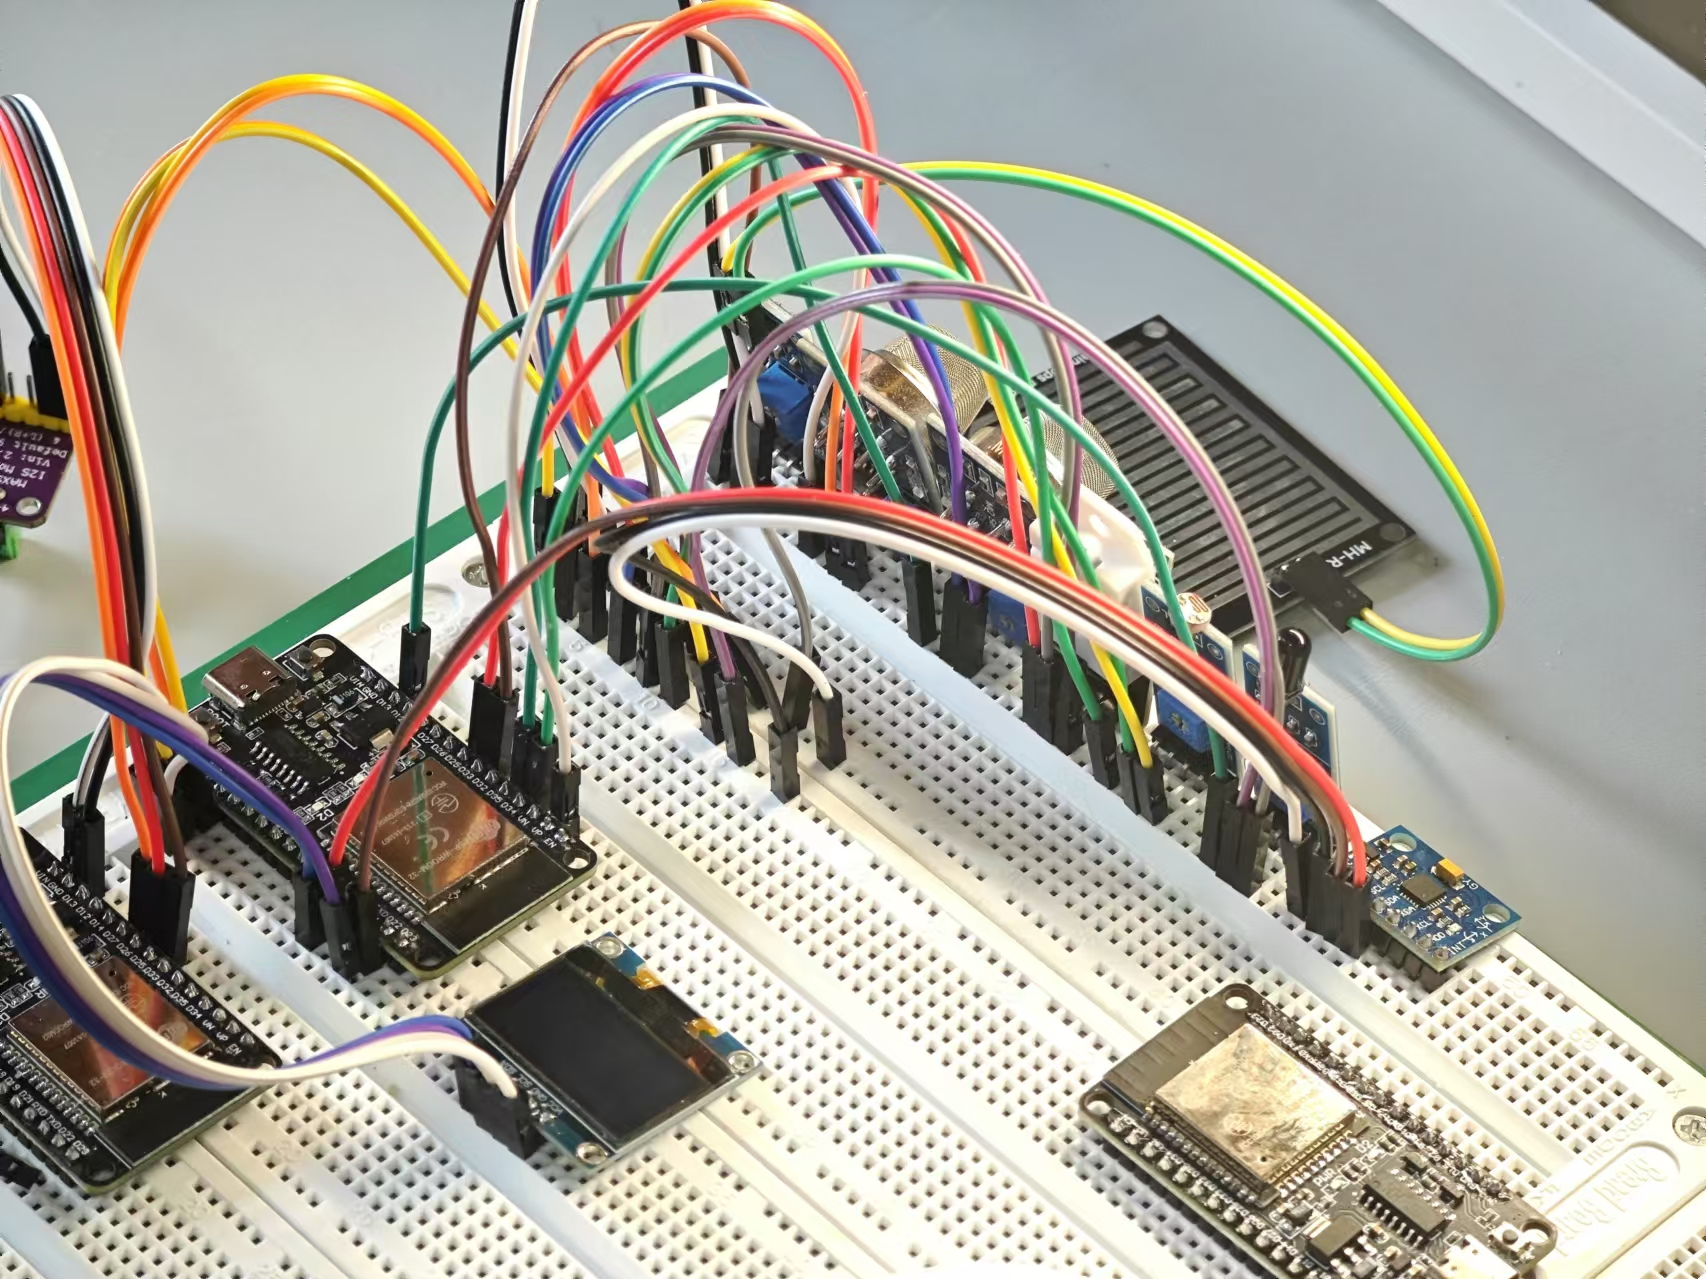
\includegraphics[width=1.0\textwidth]{BeamerImg/SlaveConn.jpg}
    \end{column}
\end{columns}
\end{frame}

\section{Progress}
\begin{frame}
  \frametitle{技术栈一:通过WebSocket连接至STT服务器}
  主要步骤:
  \begin{itemize}
    \item 1、通过HTTP GET请求获取RFC 1123时间戳
    \item 2、使用Sha-256算法对时间戳进行加密,获取鉴权地址
    \item 3、鉴权成功,握手一次,建立以WebSocket为基础的全双工通信
    \item 4、注册异步回调函数,发送base64编码语音,获取服务器返回的JSON数据
    \item 5、使用ArduinoJson库解析字符串,定义全局变量UserInput用于存储用户输入信息
  \end{itemize}
\end{frame}

\begin{frame}
  \frametitle{技术栈二:流式调用,构造JSON发送至LLM}
  \begin{columns}
    \begin{column}{0.5\textwidth}
      使用DynamicJson创建动态Json对象,按顺序构造Json即可。
        \begin{itemize}
            \item 注意到在$payload \rightarrow message \rightarrow text$中,我们可以向LLM发送多条文本,以实现多轮对话。
            \item 故可以创建一个动态数组存储多轮对话的结果,在此可以使用<Vector>
            \item 调用百度语音发声API,使用MAX98357驱动音频输出,播放语音。
        \end{itemize}
    \end{column}

    \begin{column}{0.5\textwidth}
        \centering
        \includegraphics[width=0.5\textwidth]{BeamerImg/LLMStream.jpg}
    \end{column}
\end{columns}

\end{frame}

\begin{frame}
  \frametitle{技术栈三:通过MQTT协议连接至IoT平台}
  \begin{columns}
    \begin{column}{0.6\textwidth}
      中国移动的OneNET平台专门为物联网应用开发,我们可以使用ESP32连接到MQTT服务器,之后再构建手机APP来获取数据,真正实现信息互联。
      \begin{itemize}
        \item 1、使用PubSubClient库进行MQTT通信
        \item 2、实时鉴权、连接产品ID、产品Access
        \item 3、使用HMAC-SHA256算法对消息进行签名,生成唯一Token
        \item 4、并使用MQTT协议连接至IoT平台,订阅相关主题
      \end{itemize}
    \end{column}

    \begin{column}{0.4\textwidth}
        \centering
        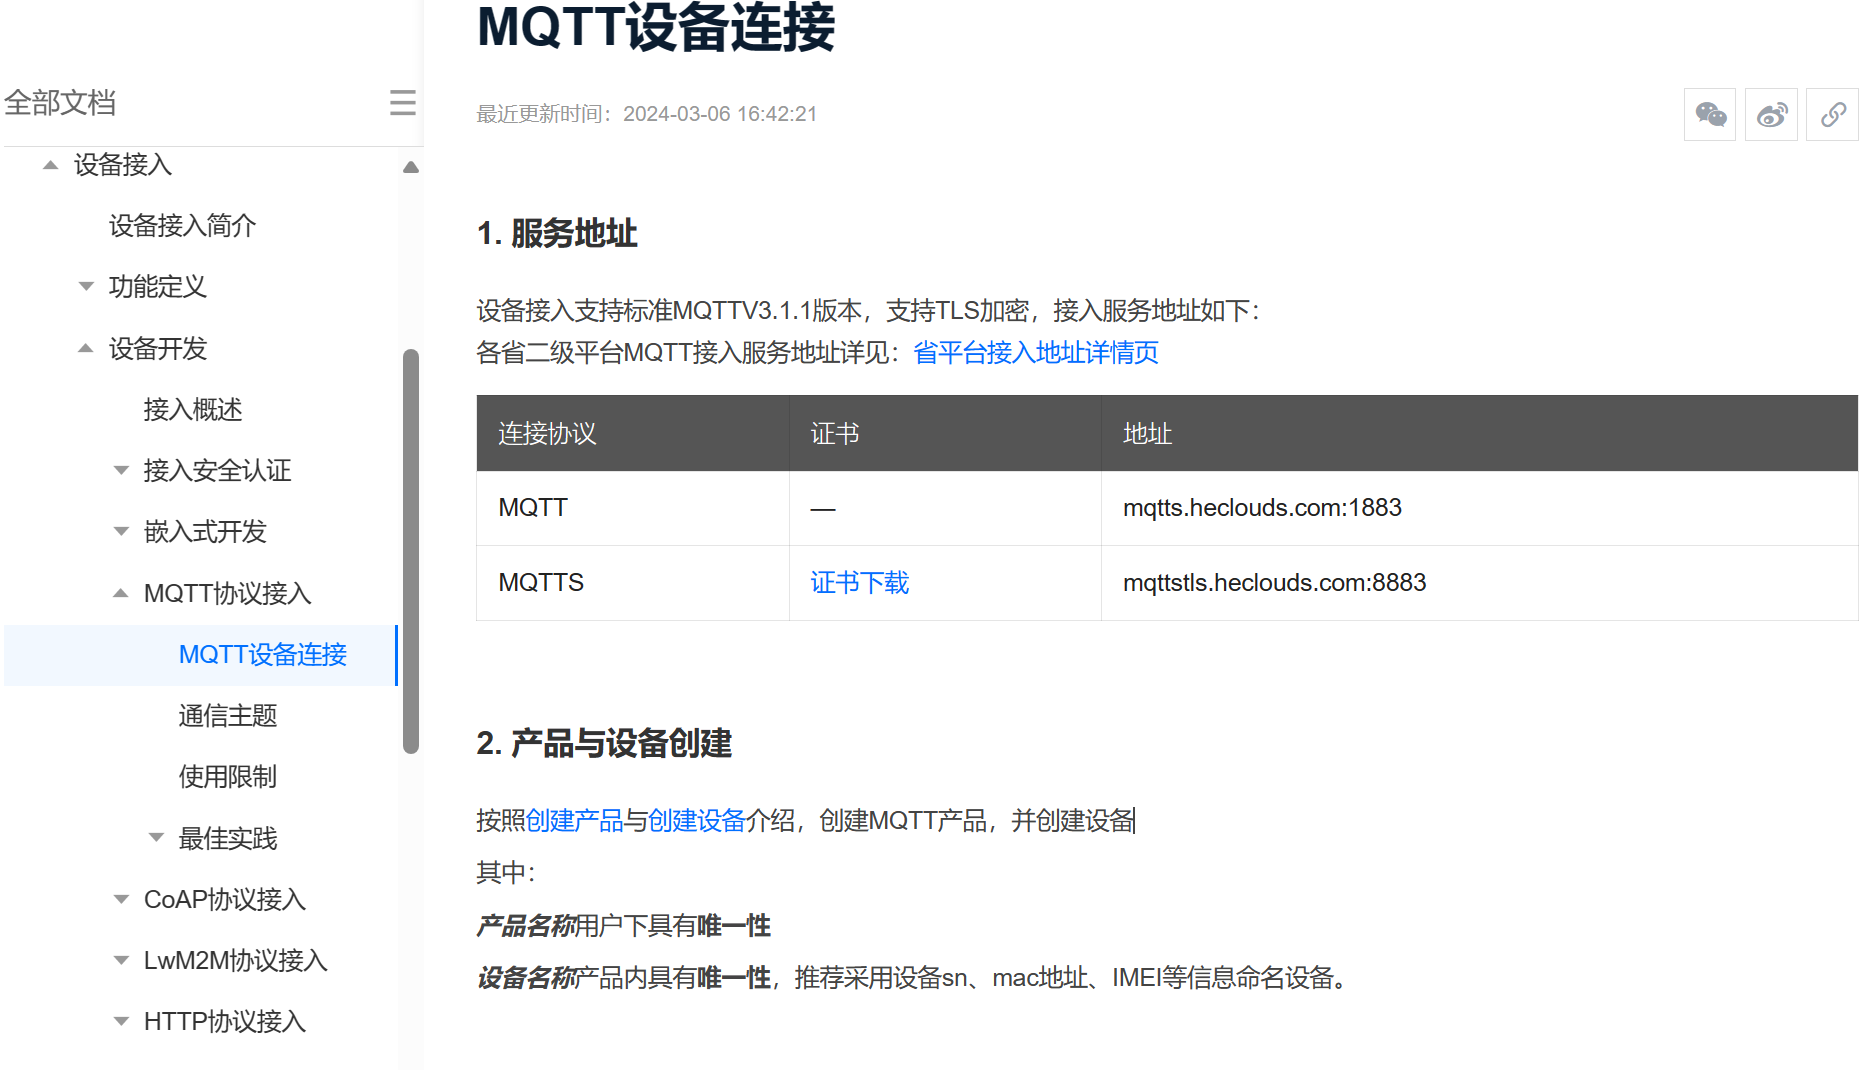
\includegraphics[width=1.0\textwidth]{BeamerImg/MQTTInit.png}
    \end{column}
\end{columns}
\end{frame}

\begin{frame}
  外接MQ135、MQ5模块
  \begin{figure} [H]
    \centering
    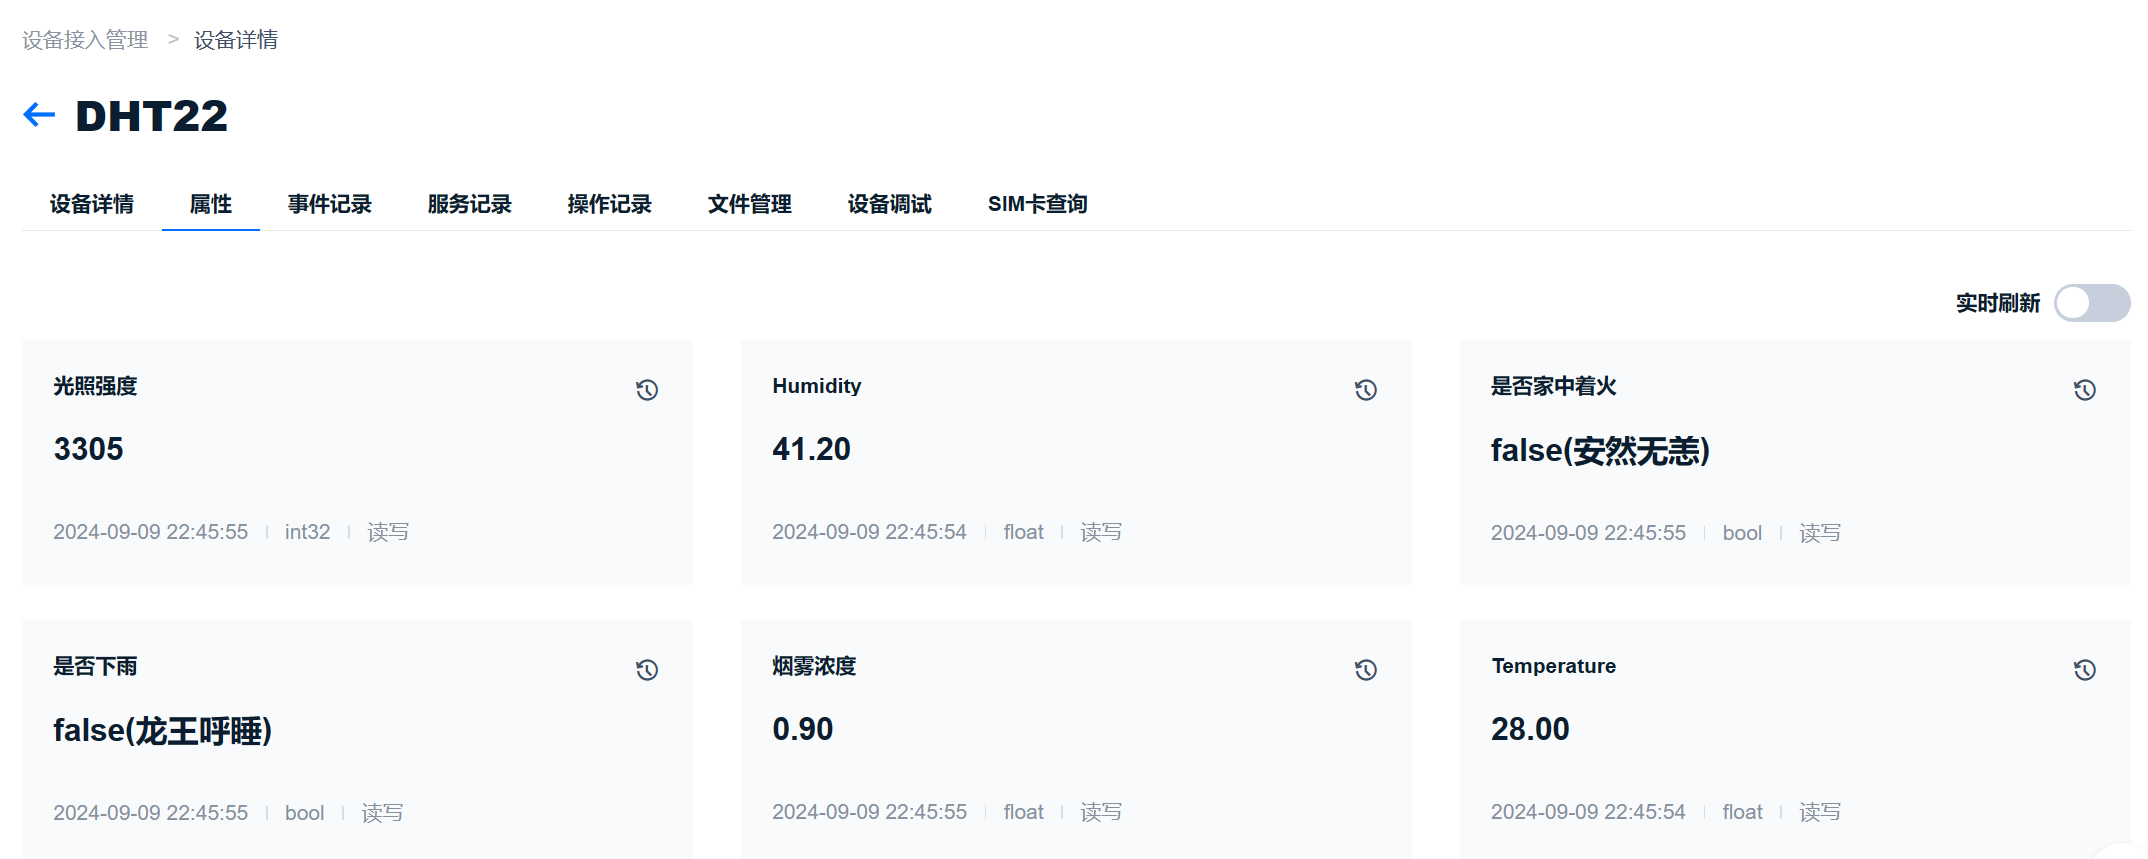
\includegraphics[width=0.9\textwidth]{BeamerImg/MQTTData.png}
    \caption{MQTT数据流}
    \label{fig:mqtt-data}
  \end{figure}
  可选数据:CO2、CO、H2、CH3COOH、CH4等
\end{frame}


\begin{frame}
  \frametitle{技术栈四:Node.js构建微信小程序}
  \begin{columns}
    \begin{column}{0.5\textwidth}
      Node.js语言用于构建网络应用程序,如服务器端的 API、实时聊天应用、单页应用等。
      \begin{itemize}
        \item 1、使用微信小程序开发工具,搭建基本框架
        \item 2、连接至MQTT服务器,实时获取数据
        \item 3、使用发布订阅模式,实现远程数据交互,远程控制家中行为等
      \end{itemize}
    \end{column}

    \begin{column}{0.5\textwidth}
        \centering
        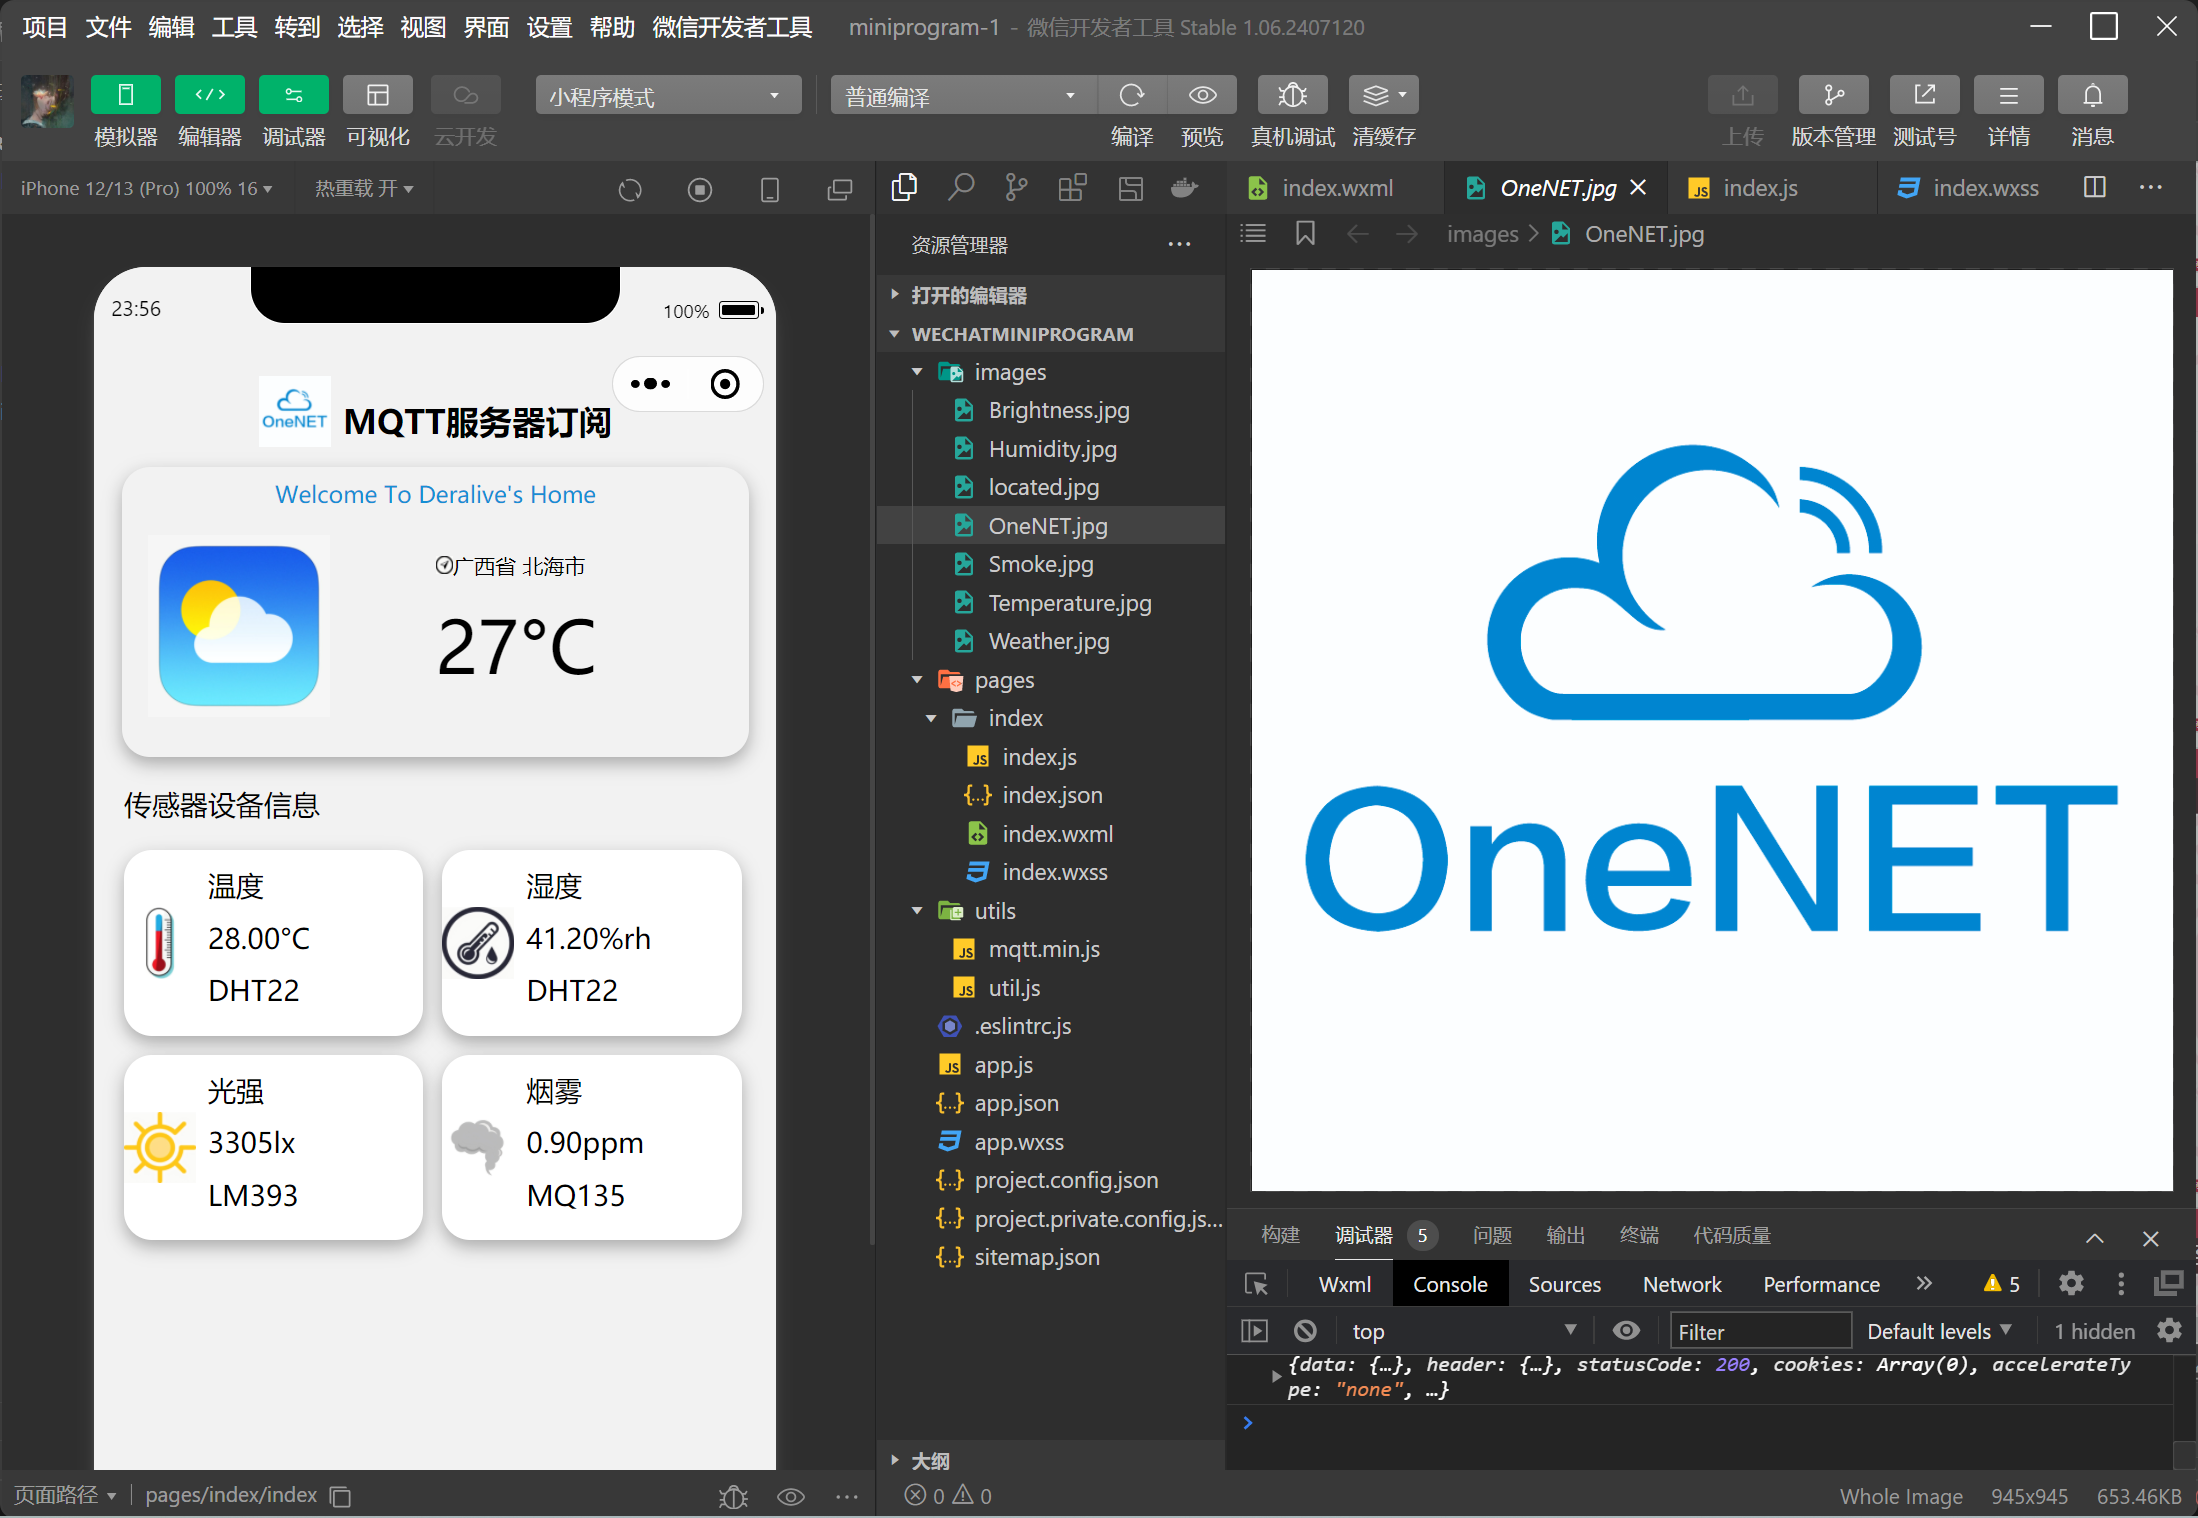
\includegraphics[width=1.0\textwidth]{BeamerImg/Wechat.png}
    \end{column}
\end{columns}
\end{frame}

\begin{frame}
  \frametitle{技术栈五:使用ESP-NOW协议实现伪AC-AP无线网络通信}
  \begin{columns}
    \begin{column}{0.5\textwidth}
      由乐鑫开发的一种低功耗、低延迟的无线通信协议,适用于 ESP 设备。
      可不占用引脚资源,构建多对多的通信网络。
      \begin{itemize}
        \item 1、设备唯一的 MAC 地址在 ESP-NOW 通信中用于标识通信目标设备
        \item 2、注册回调函数,发送结构体信息
        \item 3、使用sizeof()函数获取结构体大小,解析是哪一类信息
        \item ESP-NOW Mesh (By DALL·E) ———$\rightarrow$
      \end{itemize}
    \end{column}

    \begin{column}{0.5\textwidth}
        \centering
        \includegraphics[width=0.7\textwidth]{BeamerImg/ESP32Mesh.jpg}
    \end{column}
  \end{columns}
\end{frame}

\section{Conclusion}
\begin{frame}
  \frametitle{未来展望}
  CSI(Channel State Information)用于描述无线通信中的信道特性,可以反映出无线信号在传播过程中受到的多径、衰减、干扰等影响。CSI 在 Wi-Fi 系统中广泛应用,尤其是基于 OFDM(正交频分复用)技术的 Wi-Fi 标准,如 802.11n/ac/ax。
在这些标准中,CSI 可以用于优化传输性能、定位和环境感知等应用。

参考链接:\href{https://www.bilibili.com/video/BV1cGHreYEzB}{\underline{用 ESP32-S3 和 CSI 技术打造人体感知风扇}}

\begin{figure} [H]
  \centering
  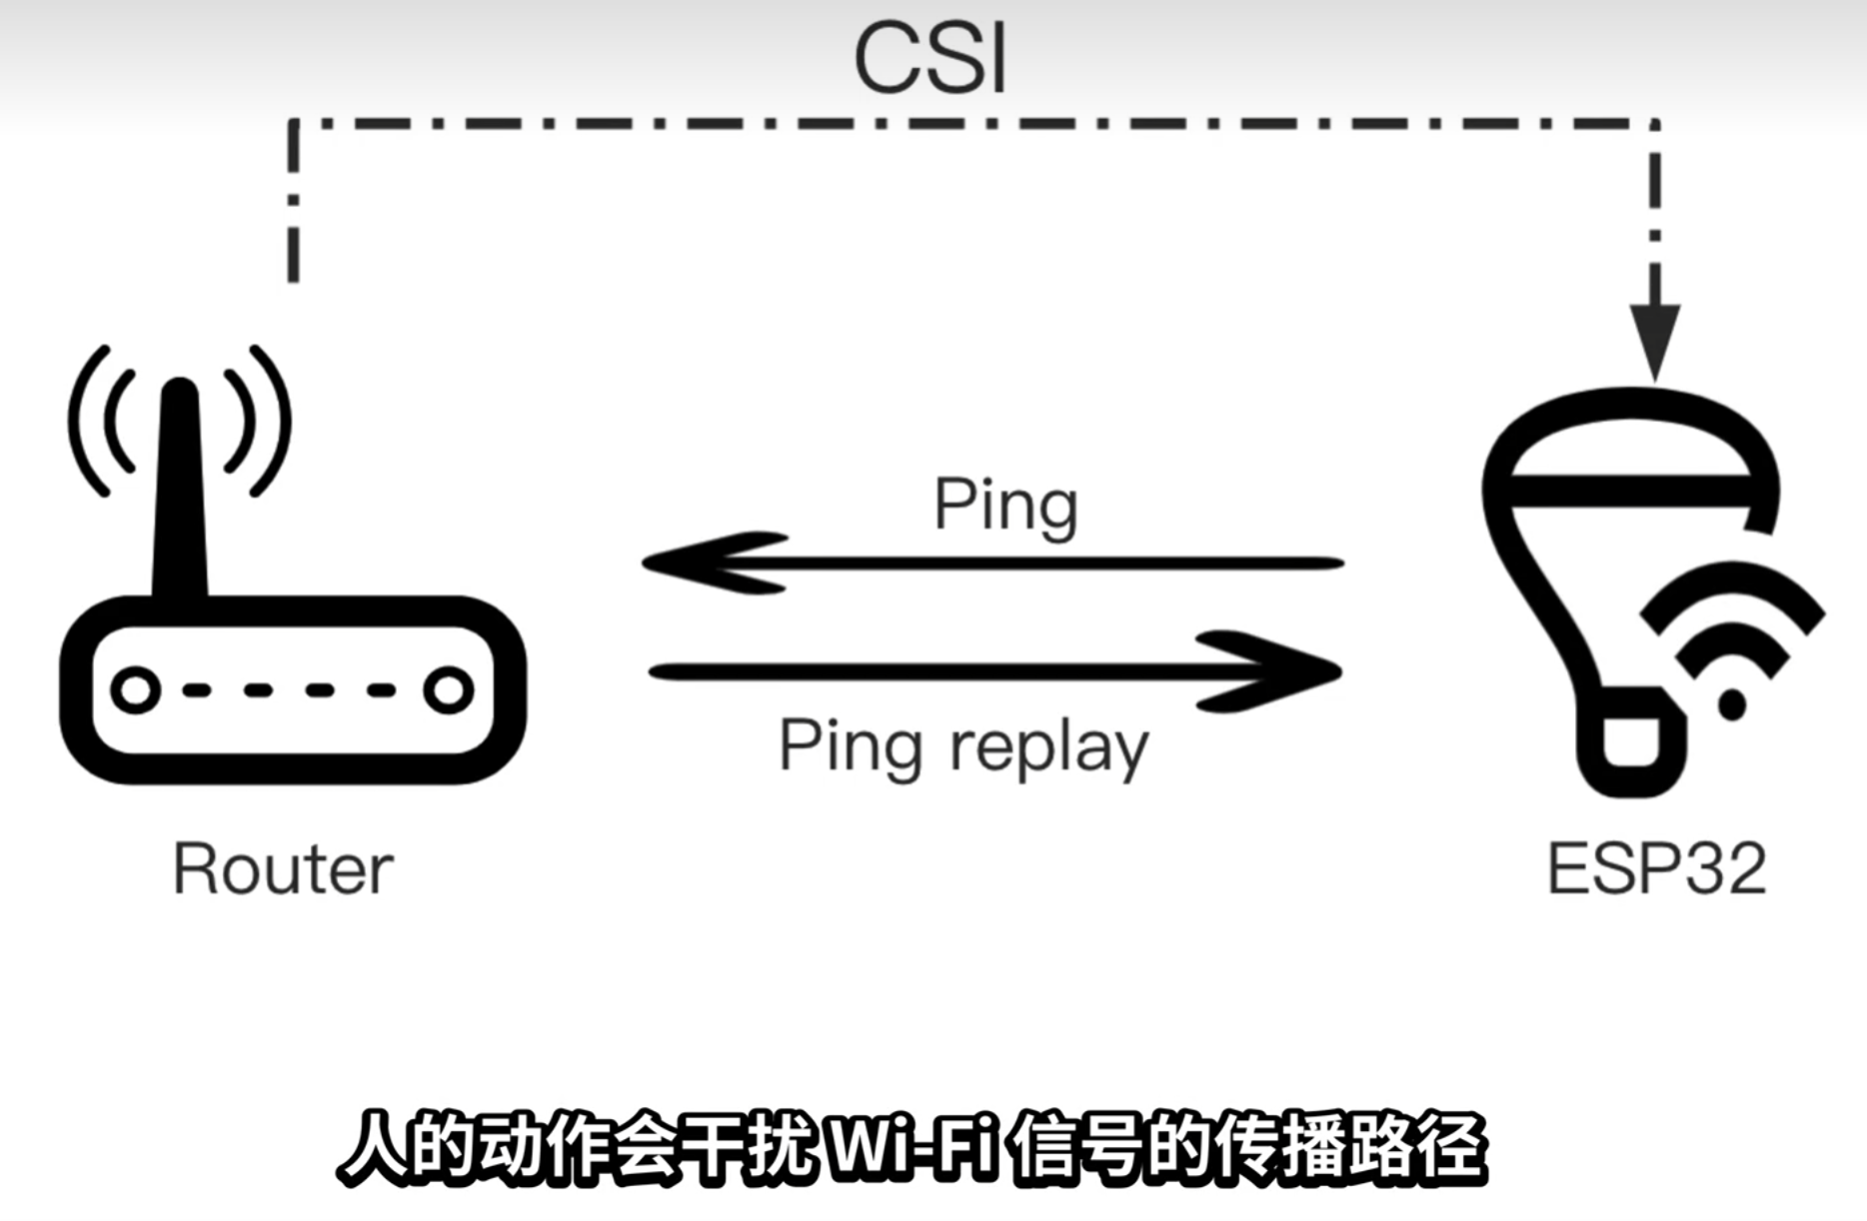
\includegraphics[width=0.6\textwidth]{BeamerImg/CSI.png}
  \caption{CSI}
  \label{fig:csi}
\end{figure}

  \noindent\textbf{Sequence Tagging Loss\\}
\end{frame}

\end{document}